TEX Toolbox: 

Citazioni:

\cite{riscv}

Immagini:

\begin{figure}[H]
  \centering
  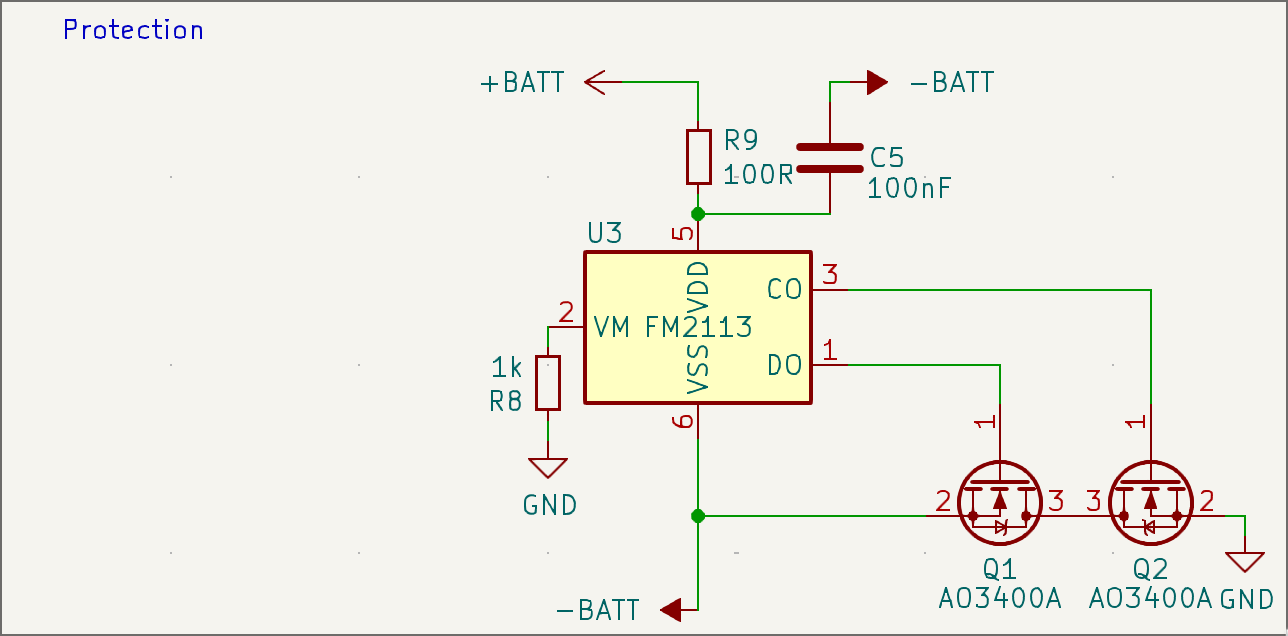
\includegraphics[width=0.8\textwidth]{images/chapter2/protection.png}
  \caption{Circuito di protezione della batteria}
  \label{fig:protection}
\end{figure}

Più immagini insieme:

\begin{figure}[H]
    \centering
    \begin{minipage}[b]{0.70\textwidth}
        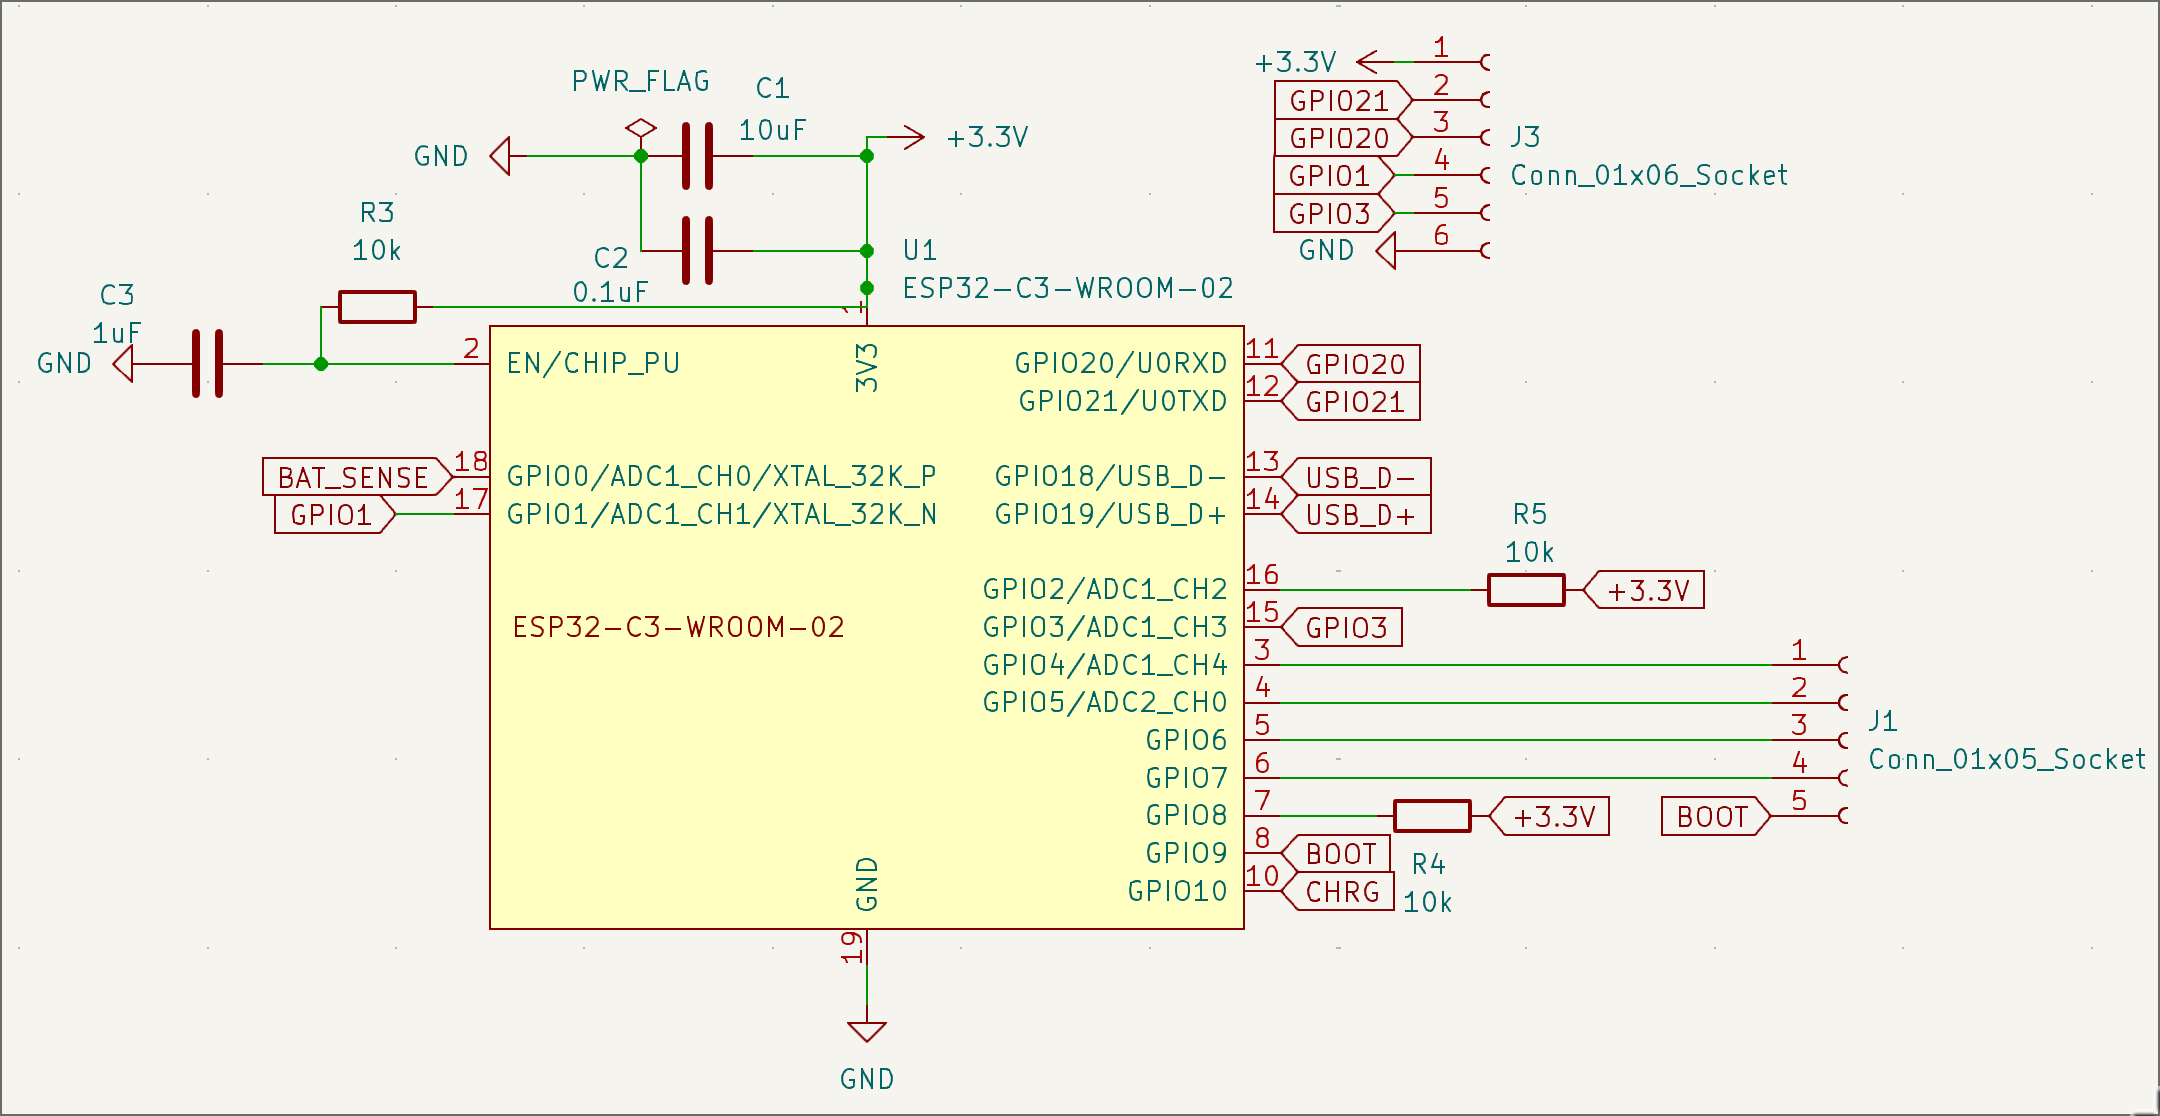
\includegraphics[width=1.0\textwidth]{images/chapter2/mcu.png}
        \caption{Collegamento del microcontrollore}
        \label{fig:mcu}  
    \end{minipage}
    \hfill
    \begin{minipage}[b]{0.28\textwidth}
        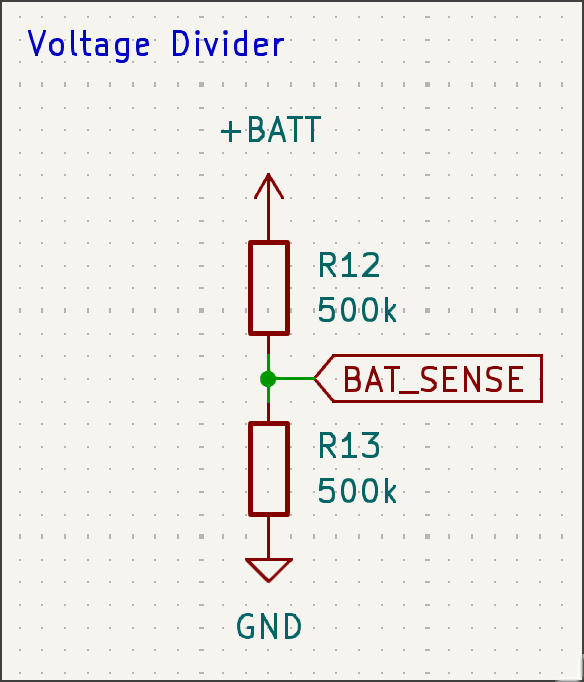
\includegraphics[width=1.0\textwidth]{images/chapter2/divider.png}
        \caption{Partitore di tensione}
        \label{fig:divider}
        \end{minipage}
\end{figure}

\begin{figure}[H]
    \centering
    \begin{minipage}[b]{0.45\textwidth}
      \includegraphics[width=1.0\textwidth]{images/chapter2/step1.jpg}
      \caption{Step 1: rimozione del processore}
      \label{fig:step1}
    \end{minipage}
    \hfill
    \begin{minipage}[b]{0.45\textwidth}
      \includegraphics[width=1.0\textwidth]{images/chapter2/step2.jpg}
      \caption{Step 2: rimozione del resistore R2}
      \label{fig:step2}
      \end{minipage}
  \end{figure}
  
  \begin{figure}[H]
    \centering
    \begin{minipage}[b]{0.45\textwidth}
      \includegraphics[width=1.0\textwidth]{images/chapter2/step3.jpg}
      \caption{Step 3: rimozione del condensatore C2 e cortocircuitazione dei pad}
      \label{fig:step2}  
    \end{minipage}
    \hfill
    \begin{minipage}[b]{0.45\textwidth}
      \includegraphics[width=1.0\textwidth]{images/chapter2/step4.jpg}
      \caption{Step 4: saldatura cavi per controllare le periferiche}
      \label{fig:step2}
        \end{minipage}
\end{figure}

Sottosezioni:

\subsection{Schema elettrico}

\subsubsection{Alimentazione}

Liste:

\begin{itemize}
    \item elemento A
    \item elemebto B
\end{itemize}


Reference to figure:

\ref{fig:federated_architecture}


Tabella:

\begin{table}[H]
    \centering
    \begin{tabular}{|c|c|c|c|}
        \hline
        \textbf{Soluzione} & \textbf{Interoperabilità} & \textbf{Velocità} & \textbf{Semplicità d'uso} \\
        \hline
        \texttt{rvsim} & 
        \begin{tabular}[c]{@{}c@{}}- Buona \\ - è possibile creare \\ syscall custom \end{tabular} & 
        \begin{tabular}[c]{@{}c@{}}- Elevata \\ - codice compilato \end{tabular} & 
        \begin{tabular}[c]{@{}c@{}}- Difficile \\ - Richiede compilazione \\ del codice\end{tabular} \\
        \hline
        \texttt{Micropython} & 
        \begin{tabular}[c]{@{}c@{}}- Scarsa \\ - difficile da integrare \end{tabular} & 
        \begin{tabular}[c]{@{}c@{}}- Buona \\ - utilizza bytecode \end{tabular} & 
        \begin{tabular}[c]{@{}c@{}}- Semplice \\ - linguaggio semplice\\ molto diffuso \end{tabular} \\
        \hline
        \texttt{rhai} & 
        \begin{tabular}[c]{@{}c@{}}- Elevata \\ - supporto a funzioni \\ e tipi custom \end{tabular} & 
        \begin{tabular}[c]{@{}c@{}}- Scarsa \\ - poco ottimizzato \end{tabular} & 
        \begin{tabular}[c]{@{}c@{}}- Semplice \\ - linguaggio minimale \end{tabular} \\
        \hline
    \end{tabular}
    \caption{Confronto tra le soluzioni di sandboxing}
    \label{tab:sandboxing_solutions}
\end{table}

Testo in evidenza:

\texttt{rhai}

Code:

\begin{listing}[H]
    \begin{minted}[
        frame=single,
        framerule=0.8pt,
        fontsize=\footnotesize,
        breaklines
      ]{rust}
    let sys_loop = EspSystemEventLoop::take()?;
    let mut peripherals = Peripherals::take().unwrap();
    let r = LedcDriver::new(
        peripherals.ledc.channel0,
        unsafe { get_ledc_timer(peripherals.ledc.timer0.clone_unchecked())? },
        peripherals.pins.gpio3,
    )?;
    ...
    let led = Arc::new(Mutex::new(Rgbw { r, g, b, a }));
\end{minted}
\end{listing}

Bibliografia esempi:

@misc{ react_website ,
    author = {Meta},
    title = {React - A JavaScript library for building user interfaces},
    howpublished = "\url{https://reactjs.org/}",
    note = {Visitato in data: 27/09/2024}
}

@article{fischer1989comparing,
  title={Comparing structured and unstructured methodologies in firmware development},
  author={Fischer, WA and Jost, JW},
  journal={Hewlett-Packard Journal},
  volume={40},
  number={2},
  pages={80--85},
  year={1989},
  publisher={HEWLETT-PACKARD CO 3000 HANOVER STREET, PALO ALTO, CA 94304}
}

@article{iee_std,
  author={},
  journal={IEEE Std 830-1993}, 
  title={IEEE Recommended Practice for Software Requirements Specifications}, 
  year={1994},
  volume={},
  number={},
  pages={1-32},
  keywords={IEEE Standards;Software;Standards organizations;Organizations;Contracts;Dams;contract;customer;prototyping;supplier;System requirements specifications},
  doi={10.1109/IEEESTD.1994.121431}
}

@misc{barile2019analisi,
  title={Analisi PESTLE Analisi SWOT},
  author={Barile, Sergio},
  year={2019},
  publisher={Tratto da https://web. uniroma1. it: https://web. uniroma1. it~…}
}

@inproceedings{al2020internet,
  title={Internet of things market analysis forecasts, 2020--2030},
  author={Al-Sarawi, Shadi and Anbar, Mohammed and Abdullah, Rosni and Al Hawari, Ahmad B},
  booktitle={2020 Fourth World Conference on smart trends in systems, security and sustainability (WorldS4)},
  pages={449--453},
  year={2020},
  organization={IEEE}
}

@misc{rfc6455,
    series =    {Request for Comments},
    number =    6455,
    howpublished =  {RFC 6455},
    publisher = {RFC Editor},
    doi =       {10.17487/RFC6455},
    url =       {https://www.rfc-editor.org/info/rfc6455},
    author =    {Alexey Melnikov and Ian Fette},
    title =     {{The WebSocket Protocol}},
    pagetotal = 71,
    year =      2011,
    month =     dec,
    abstract =  {The WebSocket Protocol enables two-way communication between a client running untrusted code in a controlled environment to a remote host that has opted-in to communications from that code. The security model used for this is the origin-based security model commonly used by web browsers. The protocol consists of an opening handshake followed by basic message framing, layered over TCP. The goal of this technology is to provide a mechanism for browser-based applications that need two-way communication with servers that does not rely on opening multiple HTTP connections (e.g., using XMLHttpRequest or \textless{}iframe\textgreater{}s and long polling). {[}STANDARDS-TRACK{]}},
}

@report{WebAssemblyCoreSpecification1,
  title = {{WebAssembly Core Specification}},
  version = {1.0},
  editor = {Rossberg, Andreas},
  date = {2019-12-05},
  institution = {{W3C}},
  url = {https://www.w3.org/TR/wasm-core-1/},
  langid = {english}
}

@cite{threejs_website,
    author = {Three.js developers},
    title = {Three.js - JavaScript 3D library},
    howpublished = "\url{https://threejs.org/}",
    note = {Visitato in data: 27/09/2024}
}

@article{oliveri2022land,
  title={In the land of MMUs: multiarchitecture OS-agnostic virtual memory forensics},
  author={Oliveri, Andrea and Balzarotti, Davide},
  journal={ACM Transactions on Privacy and Security},
  volume={25},
  number={4},
  pages={1--32},
  year={2022},
  publisher={ACM New York, NY}
}
